\documentclass[12pt]{article}

\usepackage[T1]{fontenc}
\usepackage{mathpazo}
\usepackage{eulervm}

\usepackage{amsmath}
\usepackage{amsthm}
\allowdisplaybreaks[4]
\usepackage{amssymb}

\usepackage{tikz}
\usepackage{tikz-3dplot}
\usetikzlibrary{decorations.pathreplacing, matrix}
\usepackage{nicematrix}
\usetikzlibrary{decorations.pathreplacing}
\usepackage{xy}  % Consider loading xy-pic only if needed

\usepackage{bm}
\usepackage{dcolumn} %  This package is for aligning numbers in columns, useful for tables.
\usepackage[mathscr]{eucal} % This package provides script fonts for mathematical calligraphic symbols.
\usepackage{float}  % For float placement control (e.g., [H] for "exactly here")
\usepackage{graphicx} % For including images

\usepackage{times} % This package is deprecated. Consider using a different font package if needed.
\usepackage{epstopdf} % For including EPS images (usually not needed with pdflatex)

\usepackage[square]{natbib} % Enables Author-Year citation style
\usepackage{bibentry}
\usepackage{cite} % For grouped citations like (1, 2, 3)


\usepackage{youngtab}  % For Young tableaux
\usepackage{ytableau}
\ytableausetup{mathmode, boxsize=0.9em}

\setlength{\evensidemargin}{0.3cm} % Consider unifying these lengths
\setlength{\oddsidemargin}{0.3cm}  % Consider unifying these lengths
\parskip=6pt
\frenchspacing
\textwidth=15cm
\textheight=23cm
\parindent=16pt
\topmargin=-1.2cm

% Theorem styles
\theoremstyle{definition}
\newtheorem{thm}{Theorem}[subsection]
\newtheorem{defi}[thm]{Definition}
\newtheorem{lemma}[thm]{Lemma}
\newtheorem{prop}[thm]{Proposition}
\newtheorem{coro}[thm]{Corollary}
\newtheorem{conj}[thm]{Conjecture}
\newtheorem*{pf}{Proof}

\newtheorem{ex}[thm]{Example}
\newtheorem{remark}[thm]{Remark}

\newtheorem{prob}{Problem}[subsection]

\numberwithin{equation}{subsection}

%\usepackage{hyperref}  % Load hyperref LAST (important!)


%-------------------------------------------------------------
\begin{document}


\begin{center}
{\Large\bf 
Notes on Characteristic Polytope
%and 
%Combinatorial Classes for \\[10pt]
%Restrictions of a Hyperplane Arrangement
}\\ [7pt]
\end{center}

\vskip 3mm

\begin{center}
Mingzhi Zhang
\end{center}

\vskip 3mm

\section{Characteristic Polytope}

\subsection{Characteristic Polytope of a Simplicial Complex $\Delta$}
Given a simplicial complex $\Delta$ over $[n]$, we associate to each face $\tau \in \Delta$ its characteristic vector as follows:
\[
\chi_{\tau} = (\delta_{\tau}(1), \delta_{\tau}(2), \ldots, \delta_{\tau}(n))
\]
where 
$\delta_{\tau}(i) = 
\begin{cases} 
1, & i \in \tau \\
0, & i \notin \tau
\end{cases}$.

\begin{defi}
    The \textbf{characteristic polytope} $P_{\chi}(\Delta) \subset \mathbb{R}^{n}$ of $\Delta$ is the convex hull of its characteristic vectors:
\begin{center}
    $P_{\chi}(\Delta) = \text{conv} \{\chi_{\tau} \mid \tau \in \Delta\}$.
\end{center}
\end{defi}


\begin{ex}
    $\Delta = \{\emptyset, 1, 2, 3, 12, 23 \}$, and we have the characteristic vectors:
    \begin{align*}
        \chi_{\emptyset} = (0,0,0) & \quad \chi_{1} = (1,0,0) \\
        \chi_{2} = (0,1,0) & \quad 
        \chi_{3} = (0,0,1) \\
        \chi_{12} = (1,1,0) & \quad 
        \chi_{23} = (0,1,1) \\
    \end{align*}
    Then $P_{\chi}(\Delta) = \text{conv}\{(0,0,0),(1,0,0),(0,1,0),(0,0,1),(1,1,0),(0,1,1)\}$, which is depicted as follows.
    
\tdplotsetmaincoords{70}{110}
\begin{tikzpicture}[tdplot_main_coords, scale=3.5]
    % Axes
    \draw[->] (0,0,0) -- (1.5,0,0) node[right]{$x$};
    \draw[->] (0,0,0) -- (0,1.5,0) node[right]{$y$};
    \draw[->] (0,0,0) -- (0,0,1.5) node[above]{$z$};
    
    % Points
    \coordinate (O) at (0,0,0);
    \coordinate (A) at (1,0,0);
    \coordinate (B) at (0,1,0);
    \coordinate (C) at (0,0,1);
    \coordinate (D) at (1,1,0);
    \coordinate (E) at (0,1,1);
    
    % Draw faces (filled with transparency)
    \fill[blue!20,opacity=0.3] (O) -- (A) -- (D) -- (B) -- cycle;
    \fill[red!20,opacity=0.3] (O) -- (B) -- (E) -- (C) -- cycle;
    \fill[green!20,opacity=0.3] (O) -- (A) -- (C) -- cycle;
    \fill[yellow!20,opacity=0.3] (B) -- (D) -- (E) -- cycle;
    \fill[purple!20,opacity=0.3] (C) -- (E) -- cycle;
    
    % Draw edges
    \draw[thick] (O) -- (A) -- (D) -- (B) -- cycle;
    \draw[thick] (O) -- (C) -- (E) -- (B);
    \draw[thick] (C) -- (E);
    \draw[thick] (D) -- (E);
    \draw[thick] (A) -- (C);
    
    % Label points
    \fill (O) circle (1pt) node[left] {$(0,0,0)$};
    \fill (A) circle (1pt) node[left] {$(1,0,0)$};
    \fill (B) circle (1pt) node[left] {$(0,1,0)$};
    \fill (C) circle (1pt) node[left] {$(0,0,1)$};
    \fill (D) circle (1pt) node[right] {$(1,1,0)$};
    \fill (E) circle (1pt) node[right] {$(0,1,1)$};
\end{tikzpicture}
    
\end{ex}

\begin{remark}
    It is direct to see that the characteristic vectors of 0-dimensional faces are the standard basis vectors $e_{i}$'s. In general, $\chi_{\emptyset} = \textbf{0}$ and  $\chi_{\tau} = \sum_{j \in \tau} e_{j}$ \text{for} $\emptyset \ne \tau \in \Delta$.
\end{remark}

   
% def of Chi-polytope of polytopes
\subsection{Characteristic Polytope of a Polytope Q}
Given a polytope $Q \subset \mathbb{R}^{d}$ with vertices $[n]$ , we associate to each flat $\tau$ in its lattice of flats $L_{Q}$ a characteristic vector in the same way:
\[
\chi_{\tau} = (\delta_{\tau}(1), \delta_{\tau}(2), \ldots, \delta_{\tau}(n))
\]
where 
$\delta_{\tau}(i) = 
\begin{cases} 
1, & i \in \tau \\
0, & i \notin \tau
\end{cases}$.

\begin{defi}
    The \textbf{characteristic polytope} $P_{\chi}(Q) \subset \mathbb{R}^{n}$ of $Q$ is the convex hull of its characteristic vectors:
\begin{center}
    $P_{\chi}(Q) = \text{conv} \{\chi_{\tau} \mid \tau \in L_{Q}\}$.
\end{center}

\end{defi}

\begin{ex}\label{ex4gon}
    Let $Q$ be a 4-gon, and the lattice of flats $L_{Q}$ is as follows:
    \begin{center}
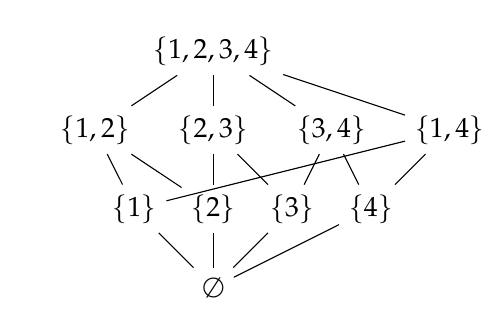
\begin{tikzpicture}
    % Define nodes
    \node (top) at (3,4) {$\{1,2,3,4\}$};

    \node (a) at (1.5,3) {$\{1,2\}$};
    \node (b) at (3,3) {$\{2,3\}$};
    \node (c) at (4.5,3) {$\{3,4\}$};
    \node (d) at (6,3) {$\{1,4\}$};

    \node (e) at (2,2) {$\{1\}$};
    \node (f) at (3,2) {$\{2\}$};
    \node (g) at (4,2) {$\{3\}$};
    \node (h) at (5,2) {$\{4\}$};

    \node (bot) at (3,1) {$\emptyset$};

    % Draw edges
    \draw (top) -- (a);
    \draw (top) -- (b);
    \draw (top) -- (c);
    \draw (top) -- (d);

    \draw (a) -- (e);
    \draw (a) -- (f);
    
    \draw (b) -- (f);
    \draw (b) -- (g);
    
    \draw (c) -- (g);
    \draw (c) -- (h);

    \draw (d) -- (h);
    \draw (d) -- (e);

    \draw (e) -- (bot);
    \draw (f) -- (bot);
    \draw (g) -- (bot);
    \draw (h) -- (bot);
\end{tikzpicture}
\end{center}
We have the corresponding characteristic vectors:
\begin{align*}
    \chi_{\emptyset} = (0,0,0,0) & \quad \chi_{12} = (1,1,0,0) \\
    \chi_{1} = (1,0,0,0) & \quad \chi_{23} = (0,1,1,0) \\
    \chi_{2} = (0,1,0,0) & \quad \chi_{34} = (0,0,1,1) \\
    \chi_{3} = (0,0,1,0) & \quad \chi_{14} = (1,0,0,1) \\
    \chi_{4} = (0,0,0,1) & \quad 
    \chi_{1234} = (1,1,1,1) \\
\end{align*}
$P_{\chi}(Q)$ is the convex hull of the above vectors and it is $4$-dimensional.
\end{ex}

% Volume and Ehrhart
\subsection{Volume and Ehrhart series}
We are mainly interested in the volume and Ehrhart seires of the characteristic polytopes. 
We list the volume and Ehrhart series of $n$-gon up to 5-gon as follows:
\begin{itemize}
    \item 3-gon: 
    \begin{align*}
    \text{vol }P_{\chi}(Q_3) &= 1, \\
    \text{Ehr}_{P_{\chi}(Q_3)}(z) &= \frac{1 + 4z + z^2}{(1 - z)^3}.
    \end{align*}
    \item 4-gon: 
    \begin{align*}
    \text{vol }P_{\chi}(Q_4) &= \frac{1}{2}, \\
    \text{Ehr}_{P_{\chi}(Q_4)}(z) &= \frac{1 + 5z + 5z^2 + z^3}{(1 - z)^4}.
    \end{align*}
    \item 5-gon:
    \begin{align*}
    \text{vol }P_{\chi}(Q_5) &= \frac{5}{24}, \\
    \text{Ehr}_{P_{\chi}(Q_5)}(z) &= \frac{1 + 6z + 11z^2 + 6z^3 + z^4}{(1 - z)^5}.
    \end{align*}
\end{itemize}

From the examples we see unimodality in the $h^*$-polynomial, and it is natural to conjecture that:
\begin{conj}
    The coefficients $h^*_{i}$ in the $h^*$-polynomial of the Ehrhart series of characteristic polytopes of $n$-gon form a unimodal sequence.
\end{conj}

\section{Characteristic Polytope of $d$-cube $\square_{d}$}

\subsection{Constructing by tensoring}
The face lattice in example \ref{ex4gon} is also the face lattice for 2-cube, and we could already see that it is hard to visualize the characteristic polytope. An algorithm to construct the characteristic polytope of $d$-cube is provided as follows.

\begin{itemize}
    \item Step 1: Start with the $(d-1)$-dim simplicial complex $\Delta$ over $[d]$. Associate each face $\tau \in \Delta$ with the corresponding standard basis vector $e_{\tau} \in \mathbb{R}^{2^d}$.
    \item Step 2: For $\sigma_{1},\sigma_{2}, \rho \in \Delta$, define 
    \begin{align*}
        e_{[\sigma_{1},\sigma_{2}]} &:= \sum_{\sigma_{1} \subset \tau \subset \sigma_{2}}e_{\tau}, \\
        e_{[\sigma_{1},\sigma_{2}]} \otimes e_{\rho} &:= e_{[\sigma_{1} \cup \rho, \sigma_{2} \cup \rho]}.
    \end{align*}
    Specifically, $e_{\emptyset} \otimes e_{\rho} = e_{\rho}$.
    \item Step 3: Let $P_{\chi}(\square_{d}) := \text{conv}\{\textbf{0}, \displaystyle \bigsqcup_{\substack{\tau \in \Delta \\ \rho \in \text{lk}_{\tau}(\Delta)}} e_{[\emptyset, \tau]} \otimes e_{\rho} \}$, and we claim that:
\end{itemize}

\begin{lemma}
    $P_{\chi}(\square_{d})$ is the characteristic polytope of the $d$-cube $\square_{d}$.
\end{lemma}
\begin{pf}
    It is direct from the construction above.
\end{pf}
% $\Delta^{\tau} := \{\rho \in \Delta \mid \rho \subset \tau\}$.
We illustrate the construction with the following example.
\begin{ex}
    Let $d = 2$, and we have the simplicial complex $\Delta = \{\emptyset, 1, 2, 12\}$. The corresponding basis vectors are:
    $e_{\emptyset} = (1,0,0,0), 
    e_{1} =(0,1,0,0), 
    e_{2} =(0,0,1,0), 
    e_{12} =(0,0,0,1)$.
    By tensoring we have:
    \begin{align*}
        &e_{\emptyset} \otimes e_{\emptyset} = e_{\emptyset} = (1,0,0,0) := v_{1} \\
        &e_{\emptyset} \otimes e_{1} = e_{1} = (0,1,0,0):= v_{2} \\ 
        &e_{\emptyset} \otimes e_{2} = e_{2} = (0,0,1,0):= v_{3} \\ 
        &e_{\emptyset} \otimes e_{12} = e_{12} = (0,0,0,1):= v_{4} \\ 
        &e_{[\emptyset, 1]} \otimes e_{\emptyset} = e_{[\emptyset, 1]} = e_{\emptyset} + e_{1} = (1,1,0,0):= v_{5} \\
        &e_{[\emptyset, 1]} \otimes e_{2} = e_{[2, 12]} = e_{2} + e_{12} = (0,0,1,1):= v_{6} \\
        &e_{[\emptyset, 2]} \otimes e_{\emptyset} = e_{[\emptyset, 2]} = e_{\emptyset} + e_{2} = (1,0,1,0):= v_{7} \\
        &e_{[\emptyset, 2]} \otimes e_{1} = e_{[1, 12]} = e_{1} + e_{12} = (0,1,0,1):= v_{8} \\
        &e_{[\emptyset, 12]} \otimes e_{\emptyset} = e_{[\emptyset, 12]} = e_{\emptyset} + e_{1} + e_{2} + e_{12} = (1,1,1,1):= v_{9} \\
    \end{align*}
    We then get the characteristic polytope $P_{\chi}(\square_{2}) = \text{conv}\{\textbf{0}, v_{i} \mid i \in [9]\}$, which is the same as in example \ref{ex4gon}.
\end{ex}

\subsection{Face vector of the characteristic polytope}
Based on the construction, we now analyze the face vector of the characteristic polytope of the $d$-cube. 

Recall that we get the characteristic polytope $P_{\chi}(\square_d)$ from the simplicial complex $\Delta_d$. By tensoring the empty set with its link in $\Delta_d$ we get the vertices of $P_{\chi}(\square_d)$, and thus we have 
\[
f_0(P_{\chi}(\square_d)) = \binom{d}{0} 2^d = 2^d.
\]
Similarly, number of $i$-faces of $P_{\chi}(\square_d)$ can be expressed as 
\[
f_i(P_{\chi}(\square_d)) = \binom{d}{i} 2^{d-i},
\]
and we have the face vector $f = (1, 2^d, \ldots, \binom{d}{i}2^{d-i}, 2d, 1)$.

\begin{remark}
    Note that $\sum_{i = 0}^{d} f_i = 3^d$, which means that $P_{\chi}(\square_d)$ has $3^d +1$ vertices.
\end{remark}

\subsection{Volume and Ehrhart series}
We have calculated the volume and Ehrhart series for $P_{\chi}(\square_2)$, which is
\begin{align*}
    \text{vol }P_{\chi}(\square_2) &= \frac{1}{2}, \\
    \text{Ehr}_{P_{\chi}(\square_2)}(z) &= \frac{1 + 5z + 5z^2 + z^3}{(1 - z)^4}.
\end{align*}
When $d = 3$, dim$P_{\chi}(\square_3) = 2^3 = 8$. Again using Mathematica and Macaulay2 we get the results as follows
\begin{align*}
    \text{vol }P_{\chi}(\square_3) &= \frac{59}{2520}, \\
    \text{Ehr}_{P_{\chi}(\square_3)}(z) &= \frac{1 + 19z + 127z^2 + 321z^3 + 329z^4 + 127z^5 + 19z^6 + z^7}{(1 - z)^8}.
\end{align*}
For $d > 3$, the computation is beyond our resource. But we notice the pattern again: the coefficients of the $h^*$-polynomial are unimodal/top-heavy. 
\begin{conj}
    The coefficients in the $h^*$-polynomial of the characteristic polytope of $d$-cube are unimodal/top-heavy.
\end{conj}

Another question is to find a formula for the volume. The characteristic polytope is similar to the \textit{independent set polytope} $I_M$ \citep{ABD10} of a matroid $M$, but it differs from $I_M$ as the latter has vertices in each slice of the hyperplane while the vertices of the former are only on certain slices.



\begin{thebibliography}{99}
\bibitem[ABD10]{ABD10} Ardila, Federico, Carolina Benedetti, and Jeffrey Doker. "Matroid polytopes and their volumes." Discrete \& Computational Geometry 43 (2010): 841-854.

\bibitem[AHK18]{AHK18} Adiprasito, Karim, June Huh, and Eric Katz. "Hodge theory for combinatorial geometries." Annals of Mathematics 188.2 (2018): 381-452.

\bibitem[Ehr62]{Ehr62} Ehrhart, Eugene. "Sur les polyèdres rationnels homothétiques à n dimensions." CR Acad. Sci. Paris 254 (1962): 616.

\bibitem[Pos09]{Pos09} Postnikov, Alexander. "Permutohedra, associahedra, and beyond." International Mathematics Research Notices 2009.6 (2009): 1026-1106.

\end{thebibliography}


\end{document}